%!TEX root = ../Thesis.tex
\chapter{Analysis}\label{cha:analysis}
This chapter contains the analysis performed on the cases specified in section \ref{sec:cases}. 


analysere time vs høgoppløyslig data. er det mulig å spore problematikken i data med kun ein sample i timen? 
Det kan eg gjere i ettermiddag! 

compare results from feature selection using unsupervised learning mehtods vs features selected using RMSE for the two needles as target variable! That should be interesting i think 



\section{Pelton needles}\label{sub:pelton_needles}
    As mentioned, there was data available from three different power plants with pelton turbines. One of plants had recorded several issues with the needle control, and was used as a case to test early detection of problems with the needle operation. 
    
    
    \begin{figure}
        \centering
        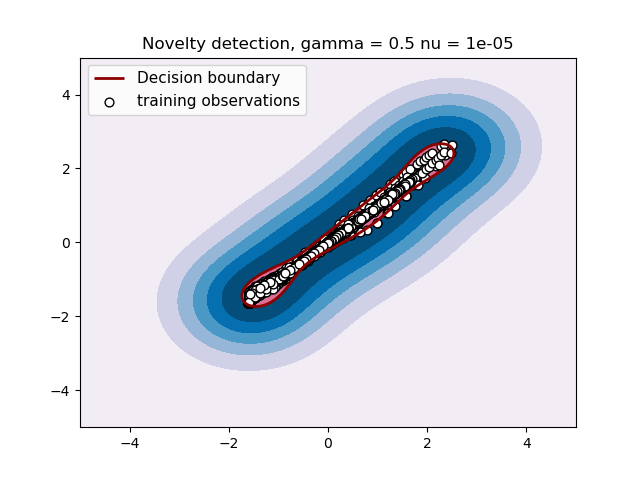
\includegraphics[scale=0.8]{report/figures/analysis/hjartdola/hjar_n2_4_novelty_05_1e-5_train.png}
        \caption{OCSVM trained on data after overhaul in Mars 2017}
        \label{fig:my_label}
    \end{figure}


    
    \begin{figure}
        \centering
        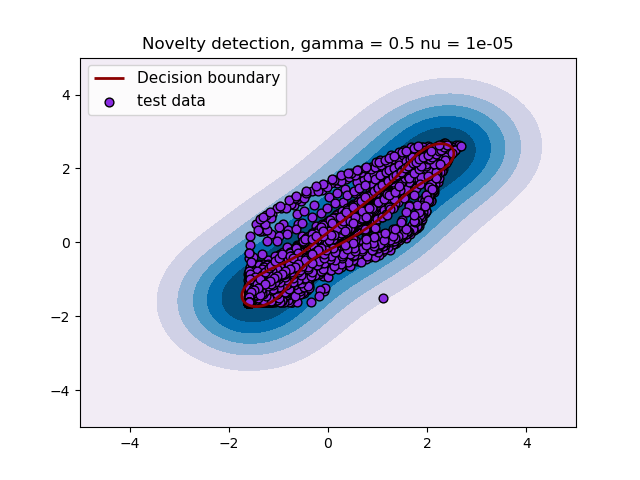
\includegraphics[scale=0.8]{report/figures/analysis/hjartdola/hjar_n2_4_novelty_05_1e-5_test.png}
        \caption{All process data from before the overhaul}
        \label{fig:my_label}
    \end{figure}



